% Insert 5
\begin{center}
    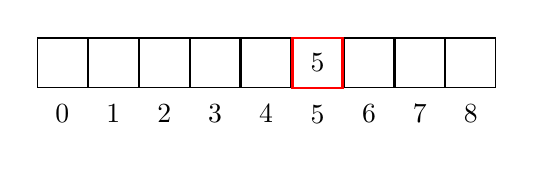
\begin{tikzpicture}
        \tikzstyle{every node}=[draw, minimum size=1.8em]
        
        \matrix[draw=none] {
            \node   (0)    [label=270:$0$] {}; & 
            \node   (1)    [label=270:$1$] {}; &
            \node   (2)    [label=270:$2$] {}; & 
            \node   (3)    [label=270:$3$] {}; &
            \node   (4)    [label=270:$4$] {}; & 
            \node   (5)    [label=270:$5$, draw=red, thick] {5}; &
            \node   (6)    [label=270:$6$] {}; &
            \node   (7)    [label=270:$7$] {}; &
            \node   (8)    [label=270:$8$] {}; \\
        };
        
    \end{tikzpicture}
\end{center}

% Insert 28
\begin{center}
    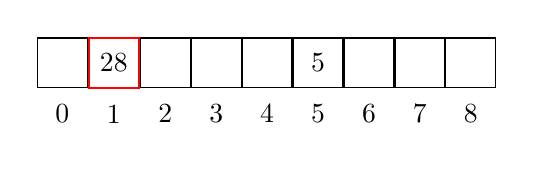
\begin{tikzpicture}
        \tikzstyle{every node}=[draw, minimum size=1.8em]
        
        \matrix[draw=none] {
            \node   (0)    [label=270:$0$] {}; & 
            \node   (1)    [label=270:$1$, draw=red, thick] {28}; &
            \node   (2)    [label=270:$2$] {}; & 
            \node   (3)    [label=270:$3$] {}; &
            \node   (4)    [label=270:$4$] {}; & 
            \node   (5)    [label=270:$5$] {5}; &
            \node   (6)    [label=270:$6$] {}; &
            \node   (7)    [label=270:$7$] {}; &
            \node   (8)    [label=270:$8$] {}; \\
        };
        
    \end{tikzpicture}
\end{center}

% Insert 19
\begin{center}
    \begin{tikzpicture}
        \tikzstyle{every node}=[draw, minimum size=1.8em]
        
        \matrix[draw=none] {
            \node   (0)    [label=270:$0$] {}; & 
            \node   (1)    [label=270:$1$, draw=red, thick] {28}; &
            \node   (2)    [label=270:$2$] {}; & 
            \node   (3)    [label=270:$3$] {}; &
            \node   (4)    [label=270:$4$] {}; & 
            \node   (5)    [label=270:$5$] {5}; &
            \node   (6)    [label=270:$6$] {}; &
            \node   (7)    [label=270:$7$] {}; &
            \node   (8)    [label=270:$8$] {}; \\
        };
        
        \node (1 1) [above=10pt of 1] {19};
        
        \draw[->, color=red] (1) -- (1 1);
        
    \end{tikzpicture}
\end{center}

% Insert 15
\begin{center}
    \begin{tikzpicture}
        \tikzstyle{every node}=[draw, minimum size=1.8em]
        
        \matrix[draw=none] {
            \node   (0)    [label=270:$0$] {}; & 
            \node   (1)    [label=270:$1$] {28}; &
            \node   (2)    [label=270:$2$] {}; & 
            \node   (3)    [label=270:$3$] {}; &
            \node   (4)    [label=270:$4$] {}; & 
            \node   (5)    [label=270:$5$] {5}; &
            \node   (6)    [label=270:$6$, draw=red, thick] {15}; &
            \node   (7)    [label=270:$7$] {}; &
            \node   (8)    [label=270:$8$] {}; \\
        };
        
        \node (1 1) [above=10pt of 1] {19};
        
        \draw[->] (1) -- (1 1);
        
    \end{tikzpicture}
\end{center}

% Insert 20
\begin{center}
    \begin{tikzpicture}
        \tikzstyle{every node}=[draw, minimum size=1.8em]
        
        \matrix[draw=none] {
            \node   (0)    [label=270:$0$] {}; & 
            \node   (1)    [label=270:$1$] {28}; &
            \node   (2)    [label=270:$2$, draw=red, thick] {20}; & 
            \node   (3)    [label=270:$3$] {}; &
            \node   (4)    [label=270:$4$] {}; & 
            \node   (5)    [label=270:$5$] {5}; &
            \node   (6)    [label=270:$6$] {15}; &
            \node   (7)    [label=270:$7$] {}; &
            \node   (8)    [label=270:$8$] {}; \\
        };
        
        \node (1 1) [above=10pt of 1] {19};
        
        \draw[->] (1) -- (1 1);
        
    \end{tikzpicture}
\end{center}

% Insert 33
\begin{center}
    \begin{tikzpicture}
        \tikzstyle{every node}=[draw, minimum size=1.8em]
        
        \matrix[draw=none] {
            \node   (0)    [label=270:$0$] {}; & 
            \node   (1)    [label=270:$1$] {28}; &
            \node   (2)    [label=270:$2$] {20}; & 
            \node   (3)    [label=270:$3$] {}; &
            \node   (4)    [label=270:$4$] {}; & 
            \node   (5)    [label=270:$5$] {5}; &
            \node   (6)    [label=270:$6$, draw=red, thick] {15}; &
            \node   (7)    [label=270:$7$] {}; &
            \node   (8)    [label=270:$8$] {}; \\
        };
        
        \node (1 1) [above=10pt of 1] {19};
        \node (6 1) [above=10pt of 6] {33};
        
        \draw[->] (1) -- (1 1);
        \draw[->, color=red] (6) -- (6 1);
        
    \end{tikzpicture}
\end{center}

% Insert 12
\begin{center}
    \begin{tikzpicture}
        \tikzstyle{every node}=[draw, minimum size=1.8em]
        
        \matrix[draw=none] {
            \node   (0)    [label=270:$0$] {}; & 
            \node   (1)    [label=270:$1$] {28}; &
            \node   (2)    [label=270:$2$] {20}; & 
            \node   (3)    [label=270:$3$, draw=red, thick] {12}; &
            \node   (4)    [label=270:$4$] {}; & 
            \node   (5)    [label=270:$5$] {5}; &
            \node   (6)    [label=270:$6$] {15}; &
            \node   (7)    [label=270:$7$] {}; &
            \node   (8)    [label=270:$8$] {}; \\
        };
        
        \node (1 1) [above=10pt of 1] {19};
        \node (6 1) [above=10pt of 6] {33};
        
        \draw[->] (1) -- (1 1);
        \draw[->] (6) -- (6 1);
        
    \end{tikzpicture}
\end{center}

% Insert 17
\begin{center}
    \begin{tikzpicture}
        \tikzstyle{every node}=[draw, minimum size=1.8em]
        
        \matrix[draw=none] {
            \node   (0)    [label=270:$0$] {}; & 
            \node   (1)    [label=270:$1$] {28}; &
            \node   (2)    [label=270:$2$] {20}; & 
            \node   (3)    [label=270:$3$] {12}; &
            \node   (4)    [label=270:$4$] {}; & 
            \node   (5)    [label=270:$5$] {5}; &
            \node   (6)    [label=270:$6$] {15}; &
            \node   (7)    [label=270:$7$] {}; &
            \node   (8)    [label=270:$8$, draw=red, thick] {17}; \\
        };
        
        \node (1 1) [above=10pt of 1] {19};
        \node (6 1) [above=10pt of 6] {33};
        
        \draw[->] (1) -- (1 1);
        \draw[->] (6) -- (6 1);
        
    \end{tikzpicture}
\end{center}

% Insert 10
\begin{center}
    \begin{tikzpicture}
        \tikzstyle{every node}=[draw, minimum size=1.8em]
        
        \matrix[draw=none] {
            \node   (0)    [label=270:$0$] {}; & 
            \node   (1)    [label=270:$1$, draw=red, thick] {28}; &
            \node   (2)    [label=270:$2$] {20}; & 
            \node   (3)    [label=270:$3$] {12}; &
            \node   (4)    [label=270:$4$] {}; & 
            \node   (5)    [label=270:$5$] {5}; &
            \node   (6)    [label=270:$6$] {15}; &
            \node   (7)    [label=270:$7$] {}; &
            \node   (8)    [label=270:$8$] {17}; \\
        };
        
        \node (1 1) [above=10pt of 1] {19};
        \node (1 2) [above=10pt of 1 1] {10};
        \node (6 1) [above=10pt of 6] {33};
        
        \draw[->, color=red] (1) -- (1 1);
        \draw[->, color=red] (1 1) -- (1 2);
        \draw[->] (6) -- (6 1);
        
    \end{tikzpicture}
\end{center}